\part{光栅化}

\chapter{光栅化}

\vspace{\baselineskip}
我们需要将上一节$[-1,1]^3$的立方体内的物体绘制到屏幕上, 我们对屏幕的定义如下: 

\begin{enumerate}[itemsep=-0.5em]
	\item 屏幕是像素的数组; 
	\item 分辨率是屏幕像素数组的尺寸; 
	\item 屏幕是光栅成像设备. 
\end{enumerate}

\textbf{光栅化 (Rasterization) }指的是将物体绘制到屏幕上. \textbf{像素 (Pixel) }是具有统一颜色的小方块, 是由不同颜色组合而成的 (例如RGB) . 

\section{屏幕空间}

\begin{figure}[H]
	\centering
	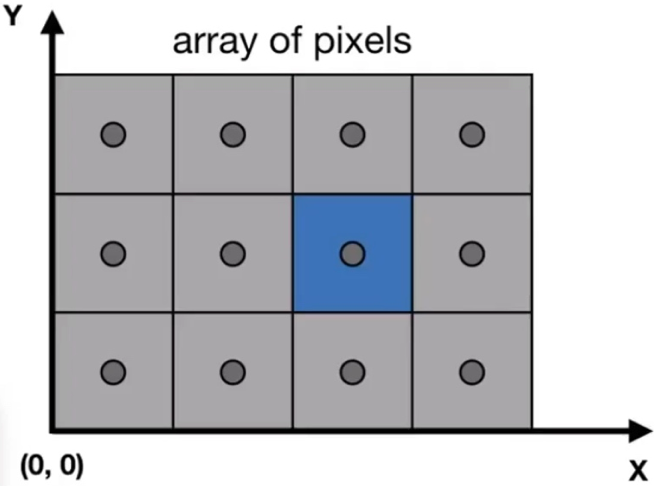
\includegraphics[scale=.3]{pingmukongjian.png}
	\caption{屏幕空间示意图}
	\label{fig:projection}
\end{figure}

我们认为屏幕左下角为原点, 向右为x轴, 向上为y轴. 建立平面直角坐标系. 屏幕空间满足以下几点: 

\begin{enumerate}[itemsep=-0.5em]
	\item 我们认为像素坐标$(x,y)$为整数坐标; 
	\item 像素坐标覆盖范围为$(0,0)$到$(\text{width}-1,\text{height}-1)$; 
	\item 像素的中心点在$(x+0.5,y+0.5)$; 
	\item 整个屏幕的覆盖范围在$(0,0)-(\text{width}, \text{height})$.
\end{enumerate}

我们需要从$[-1,1]^2$变换到$[0,\text{width}]\times[0,\text{height}]$. 这里只需要一个拉伸变换, 变换矩阵为: 

\begin{equation}
	M_{viewpoint}=\begin{pmatrix}
		\frac{width}{2} &0&0&\frac{width}{2}\\
		0&\frac{height}{2}&0&\frac{height}{2}\\
		0&0&1&0\\
		0&0&0&1
	\end{pmatrix}
\end{equation}

\section{三角形的光栅化}

对于一个$3$维图形我们可以用三角形去表示一个一个小面. 使用三角形的主要原因是: 

\begin{itemize}[itemsep=-0.5em]
	\item 三角形是最基本的多边形; 
	\item 任何多边形都可以拆分成三角形; 
	\item 空间内任何三个点的连线一定是平面; 
	\item 三角形由清晰的内部和外部定义; 
	\item 三角形只要定义顶点的属性就可以计算三角形内部点的渐变关系 (三角形的内部插值) . 
\end{itemize}

对于一个三角形, 如何映射在像素空间上问题, 可以转换成判断一个像素和三角形的位置关系. 最简单的方法就是进行\textbf{离散化 (Sampling) }. 采样就是连续函数的离散化过程. 代码表示如下: 

\begin{lstlisting}]
for(int x = 0; x < max; ++x)
	output[x]=f(x);
\end{lstlisting}
我们对于给定三角形, 判断像素中心是否在三角形内部. 如果在, 那么这个点为$1$, 否则为$0$.

\begin{equation}
	\text{inside}(t, x, y)=\left\{\begin{matrix}
		1 & \text{point}(x,y)\ \text{in triangle}\ \mathcal{t}\\ 
		0 & \text{otherwise}
	\end{matrix}\right.
\end{equation}

判断代码就可以写为: 
\begin{lstlisting}]
for(int x = 0; x < xmax; ++x)
	for(int y = 0; y < ymax; ++y)
		image[x][y] = inside(tri, x+0.5, y+0.5);
\end{lstlisting}

对于像素是否在三角形内部的判断, 可以使用叉积. 具体可以在叉积的讲解部分查看. 

对于在边界上的三角形点, 本门课不做处理 (可以根据具体情况具体分析) . 为了能够更快速的遍历像素点, 我们可以用以下方法: 

\begin{itemize}[itemsep=-0.5em]
	\item 使用包围盒 (Bounding box) , 只对三角形最大的包围矩形区进行遍历. 但是不适用于窄长的三角形. 
	\item 找到每一行三角形包围住最左和最右边的点进行遍历. 
\end{itemize}

我们的结果可能会生成大量的锯齿, 此时我们需要一些方式来消除锯齿. 

\chapter{反走样}
在上一章中我们通过采样的方式把一个三角形变成离散的点显示在屏幕上. 但是我们会发现我们产生的图片具有很多的锯齿. 因此如何消除这些锯齿, 我们就要引入\textbf{反走样 (Antialias) }技术. 

\section{瑕疵}
在采样的过程中, 我们会产生许多的锯齿. 这些锯齿的学名就叫做\textbf{走样 (Alias) }. 之所以会产生走样的原因是因为信号的变化速度比较快 (高频信号) , 但是我们的采样比较慢 (低频采样) . 常见的走样分为以下几种: 
\begin{itemize}
	\item 锯齿: 空间上采样产生的走样; 
	\item 摩尔纹: 空间上下采样产生的走样; 
	\item 车轮效应: 时间上采样产生的走样. 
\end{itemize}
这些我们也会称为采样的\textbf{瑕疵 (Artifacts) }. 

\section{反走样方法}
为了能够减轻走样带来的影响, 我们会对要采样的图形先进行模糊操作, 再根据模糊后的图形进行采样, 这就是反走样的过程. 
\begin{figure}[H]
	\centering
	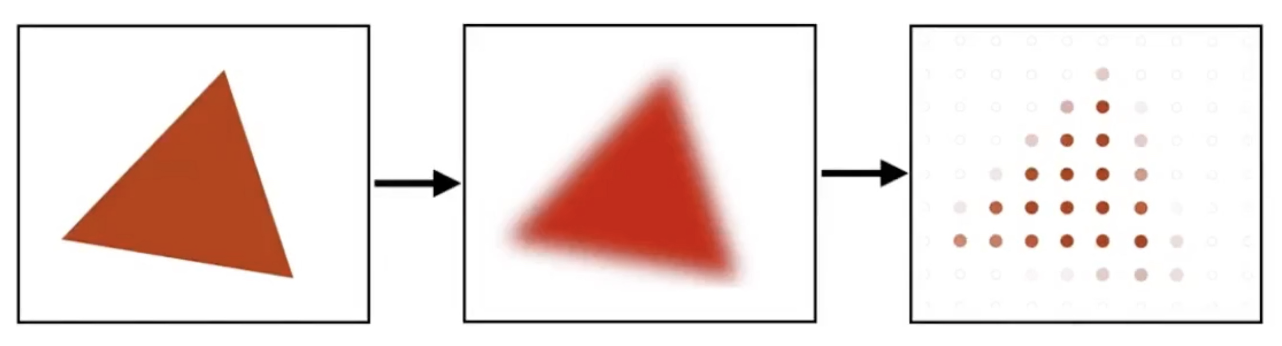
\includegraphics[scale=.3]{antialias.png}
	\caption{反走样过程示意}
	\label{fig:antialias}
\end{figure}

\section{走样产生的原因}
\subsection{傅立叶变换}
任何一个信号都可以表示为一些正弦波和余弦波以及常数的线性表示, 我们称之为\textbf{傅立叶展开}. 而\textbf{傅立叶变换}指的是将一个时域上的信号转换到频域的过程. 
\subsection{走样和滤波}
走样更为学术的定义应该是两个不同频率的信号在使用相同采样的方法后产生的结果无法进行区分. 
\begin{figure}[H]
	\centering
	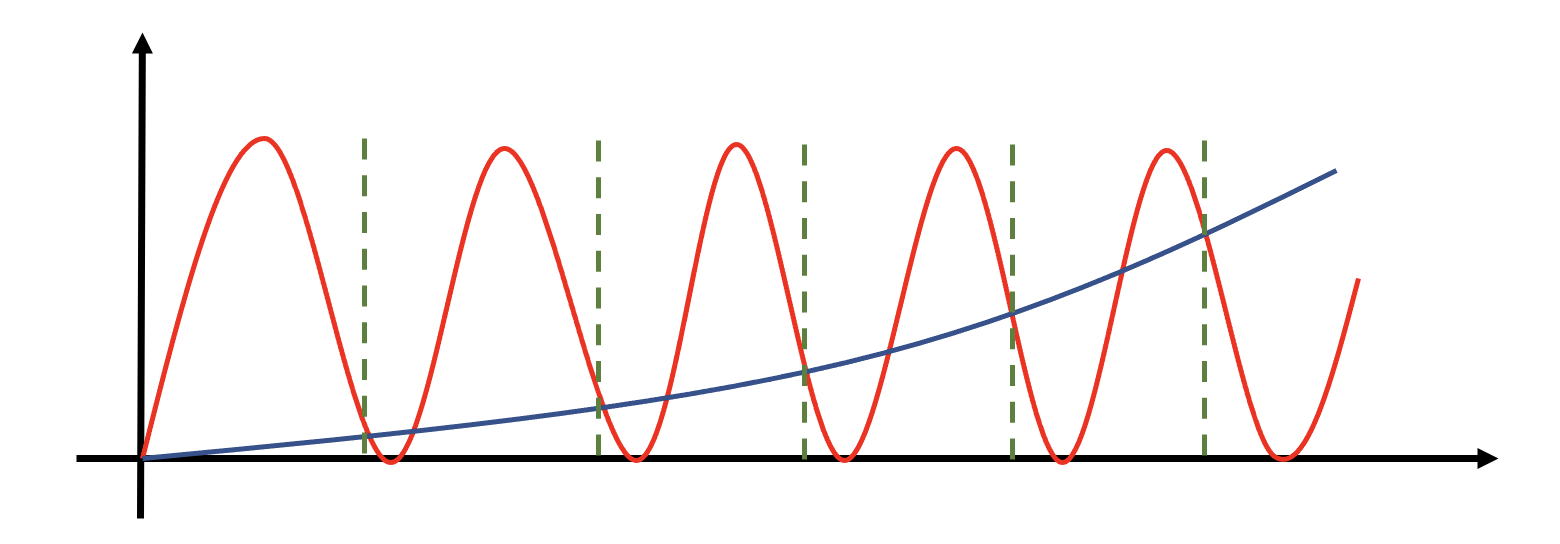
\includegraphics[scale=.3]{caiyang.png}
	\caption{走样示意图}
	\label{fig:alias}
\end{figure}
图中的红色信号和蓝色信号是两个频率不一样的信号, 绿色虚线处是采样点, 我们发现两个不同频率的信号在同一个采样方式下结果相同, 这就产生了走样. 

\textbf{滤波 (Filter) }是把特定频率的波过滤掉. 如果仅保留高频信息, 那么这称为高通滤波; 如果仅保留低频信息称为低通滤波; 如果既删除高频信息, 还删除低频信息, 只保留中频信息称为带通滤波. 

\begin{figure}[H]
	\centering
	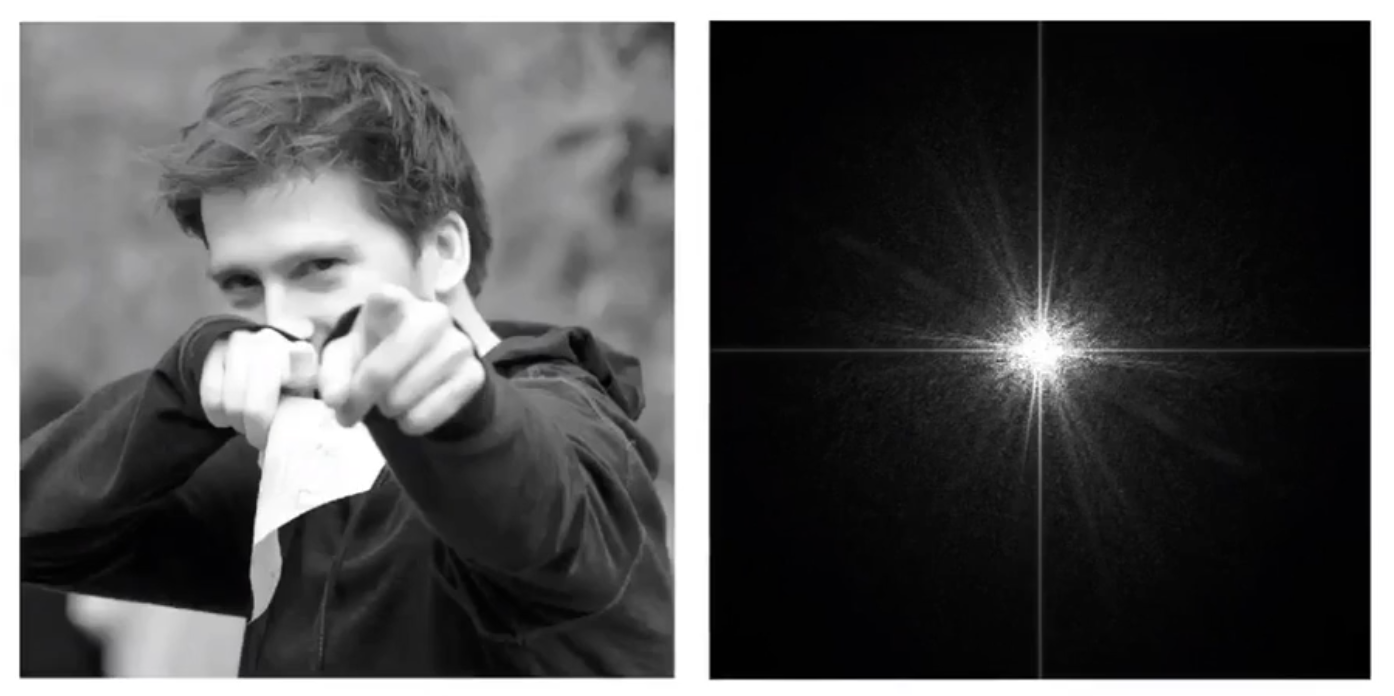
\includegraphics[scale=.3]{fuliye.png}
	\caption{傅立叶变换示意图}
	\label{fig:fuliye}
\end{figure}
对于一个图片我们进行傅立叶变换后, 得到的是上面右图的样子. 我们进行解释: 中心代表了低频信息, 边缘代表了高频信息, 亮度代表对应频率的能量. 对于图片而言, 一般低频信息更加的丰富, 而高频信息比较少. 高频信息一般代表\textbf{边缘信息}, 因为边缘信息频率比较高; 低频信息是图片\textbf{模糊后的结果}, 频率变化小. 
\begin{question}
\textbf{为什么傅立叶变换后图片有一束明显的十字交叉?}

傅立叶变换中我们会认为图片是“连续”的. 我们会在原图上下左右不断重复图片以达到“连续”的效果. 而图片的四周一般变换非常的快, 属于高频的信息, 对应在频谱图上就是会有一束明显的十字交叉, 代表了高频的边缘信息. 
\end{question}

\section{卷积和卷积定律}
滤波可以看作卷积操作, 也可以看作平均操作. \textbf{卷积 (Convolution) }操作是用一个卷积核在信号上不断地滑动, 每一次卷积操作的结果是卷积核和对应位置信号乘积的和, 可以看作一次加权平均的过程. 

\begin{titledbox}{卷积定律}
	\centering 时域上的卷积等于频域上的乘积

    \centering 频域上的乘积等于等于频域上的卷积
\end{titledbox}

\subsection{Box Filter}
\textbf{Box Filter}是一个格式如下的滤波器: 
\begin{equation}
	\frac{1}{n^2} X^{n\times n}
\end{equation}
其中, $X$是一个$n \times n$大小的全$1$矩阵. 这个卷积核对临近的$n\times n$的像素做平均. $n$越大, 滤波器得到的频率范围越低. 

\subsection{深入了解采样}
采样我们可以认为是一个连续函数乘以一系列的脉冲函数的结果. 根据卷积定律我们知道, 这相当于连续函数的傅立叶变换和脉冲函数傅立叶变换的卷积. 脉冲函数的傅立叶变换还是脉冲函数. 卷积的结果是信号的频谱在不断地重复. 
我们可以总结得出, 采样就是在重复一个原始信号的频谱. 

\begin{figure}[H]
	\centering
	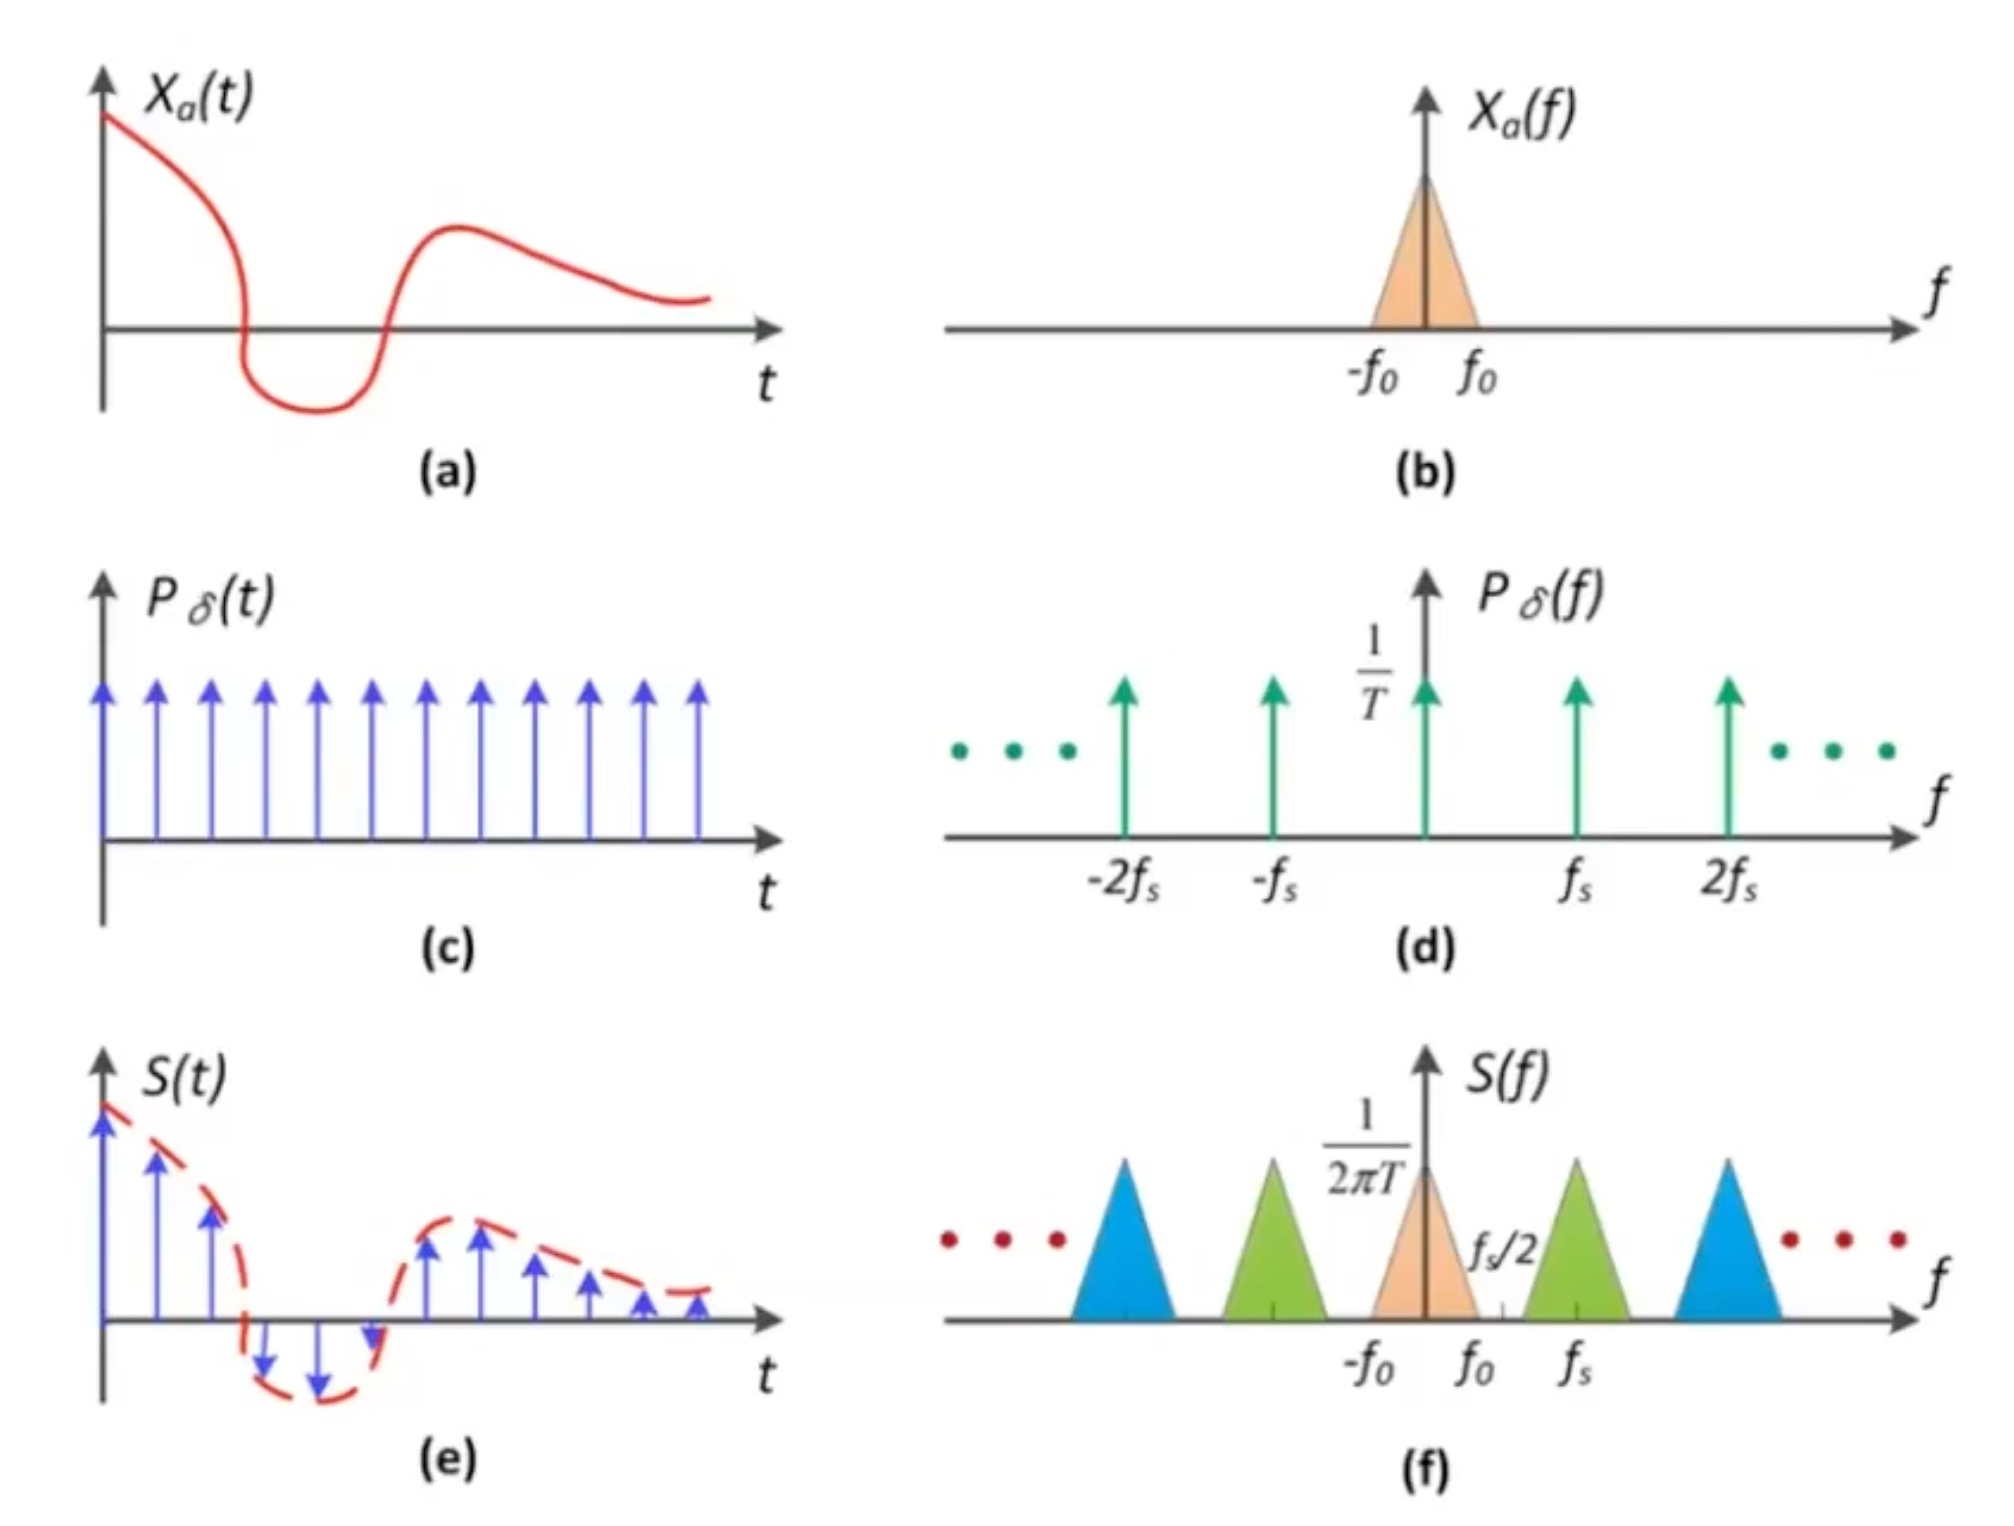
\includegraphics[scale=.15]{caiyang1.png}
	\caption{采样示意图}
	\label{fig:caiyang}
\end{figure}
当采样率不足时会使得频谱之间的间隔太小, 导致频谱间产生重叠, 这些重叠就是走样. 

\begin{figure}[H]
	\centering
	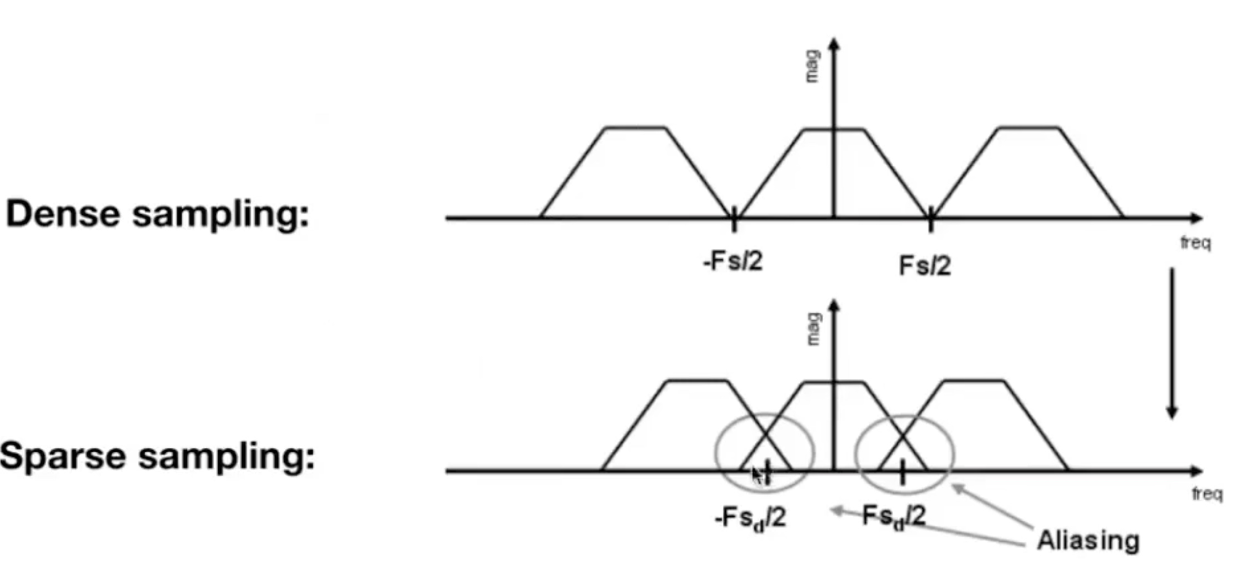
\includegraphics[scale=.4]{pinpuzouyang.png}
	\caption{频谱重叠示意图}
	\label{fig:pinpuzouyang}
\end{figure}

这也就解释了为什么使用高通滤波器可以帮助我们减少走样. 这是因为使用高通滤波器只保留更窄的频率范围, 可以减少频谱的重叠. 

\section{反走样的方法}
目前常用的反走样方法有两种: 
\begin{itemize}
	\item 提高采样率 (分辨率) . 这是从物理层面上提高采样率来减少走样的方式, 但是不够实用; 
	\item 先进行模糊操作, 再进行采样的操作, 也就是我们之前所介绍的反走样方法. 
\end{itemize}

在实际的操作中, 我们使用MSAA (Multi-Sampling Antialiasing) 的方式来近似进行反走样的操作, 具体的步骤如下: 
\begin{enumerate}
	\item 把每一个像素点拆分成$n\times n$的小像素点; 
	\item 对每一个小像素点判断该点是否在图形中; 
	\item 每一个像素点的结果都是这些小像素点的平均结果. 
\end{enumerate}
MSAA仅仅指的是模糊的过程, 并不包含采样的过程. 这样的方法虽然简单, 效果好, 但是会增加计算量. 在工业界中, 一般会采用更为有效的方式拆分采样点, 甚至会复用采样点以达到更好的效果. 

除此之外, 目前业界还有一些其他的方式进行反走样: 
\begin{itemize}
	\item FXAA (Fast approximate AA) 是通过后期处理的方式处理锯齿. 先得到已经有锯齿的图像, 找到边界后替换成没有锯齿的边界; 
	\item TAA (Temporal AA) 是通过抖动的方式进行多次采样, 将多个帧合成就相当于多次采样. 
\end{itemize}

\section{超分辨率*}
\textbf{超分辨率 (Super Sampling) }指的是将一个分辨率较小的图片还原成分辨率较大的图片. 和反走样虽然意义不同, 但是任务类似. 对于超分辨率问题, 最重要的是猜测缺失像素的内容, 比较适合使用神经网络DLSS (Deep-learning Super Sampling) 进行预测. 

\section{可见性与遮挡性}
当我们有多个在不同位置的三角形需要进行光栅化的时候, 我们需要知道直接三角形的前后关系保证在后面的会被前面的图形遮挡. 因此我们需要一定的算法保证前面的图形可以遮挡后面的图形. 

\subsection{画家算法}
\textbf{画家算法 (Painter's Algorithm) }指的是使用油画的方式进行渲染. 我们先光栅化比较远图形, 然后光栅化前面的图形进行覆盖. 
也就是说, 后画的东西会覆盖掉以前画的东西.

使用这个算法我们需要先对所有的三角形按照远近排序, 然后从远到近进行光栅化. 对三角形远近的排序的时间复杂度为$O(n\log n)$.这种方法有以下几个问题: 
\begin{itemize}
	\item 算法复杂度比较高, 并且有时候不好确定各个三角形的远近; 
	\item 如果出现互相遮挡的情况形成了一个环, 那么采用画家算法失效. 
	\begin{figure}[H]
		\centering
		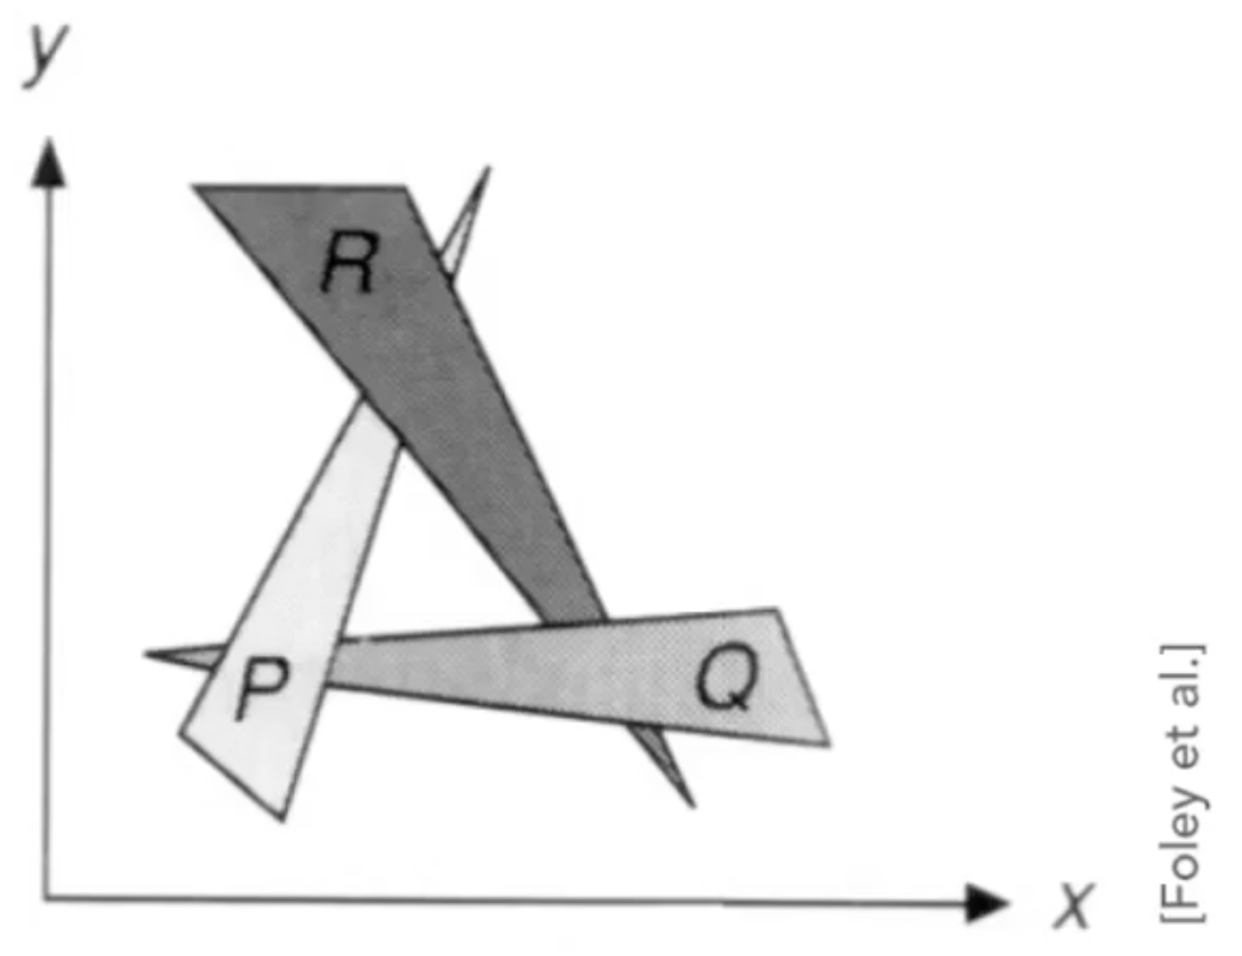
\includegraphics[scale=.2]{huajiasuanfa.png}
		\caption{遮挡成环的情况}
		\label{fig:zhedang}
	\end{figure}
	
\end{itemize}

\subsection{Z Buffer}
我们引入了\textbf{深度缓存技术 (Z Buffer) }, 记录每一个像素总最近的距离. 会生成深度缓存 (Depth buffer) 和颜色缓存 (Frame buffer) . 对于任何一个像素, 我们通过遍历所有三角形上包含了这点的点选择最近的点保存深度信息和颜色信息. 
Z Buffer的算法如下: 
\begin{lstlisting}
for(each triangle T)
	for(each sample (x,y,z) in T)
		if(z < zbuffer[x,y])
			framebuffer[x,y] = rgb; // 更新颜色
			zbuffer[x,y] = z;       // 更新深度值
		else
			;                       // 什么也不做
\end{lstlisting}
深度缓存技术的时间复杂度是$O(n)$. 这并不是一个排序算法, 因此复杂度比排序算法要小.

如果MASS中需要深度缓存技术, 需要对每一个采样点使用Z Buffer算法. 
